\section{Natural Language
Processing (NLP)}
NLP è l'intersezione tra computer science(AI) e lo studio delle lingue.

In generale ci si riferisce a migliorare la comunicazione tra uomo e macchina.

Però NLP viene usato anche per analizzare tanti documenti per fornire informazione.


\subsection{Task comuni per NLP}
\begin{itemize}
    \item riconoscimenti del parlato(determinare il testo da audio)
    \item Sentiment analysis(analisi della polarità del testo), una
    variate si chiama analisi delle emozioni
    \item divisione dell'argomento e riconoscimento(dato del tesot, lo divide in segmenti
    e li categorizza per argomento)
    \item image captioning: data un'immagine. descrivere quello che c'è
    \item riassumere testi/documenti: genera un nuovo documento con poca perdita di
    informazione
    \item Document similarity: capire quanto sono simili due documenti
    \begin{itemize}
        \item Similarità di Jaccard
        \item \begin{equation}
                  Jaccard = \frac{intersection(A,B)}{union(A,B)}
        \end{equation}
        \item Si possono usare le reti neurali per \textbf{Representation Learning}
        dove ogni parola diventa parte del vettore che rappresenta il documento, poi
        si può calcolare la \textbf{Cosine Similarity}.
    \end{itemize}
    \item
\end{itemize}

Un modo per fare sentiment analisis è fare un classificatore gerarchico,
solitamente il classificatore gerarchico è meglio di un solo strato.

\begin{figure}[H]
    \centering
    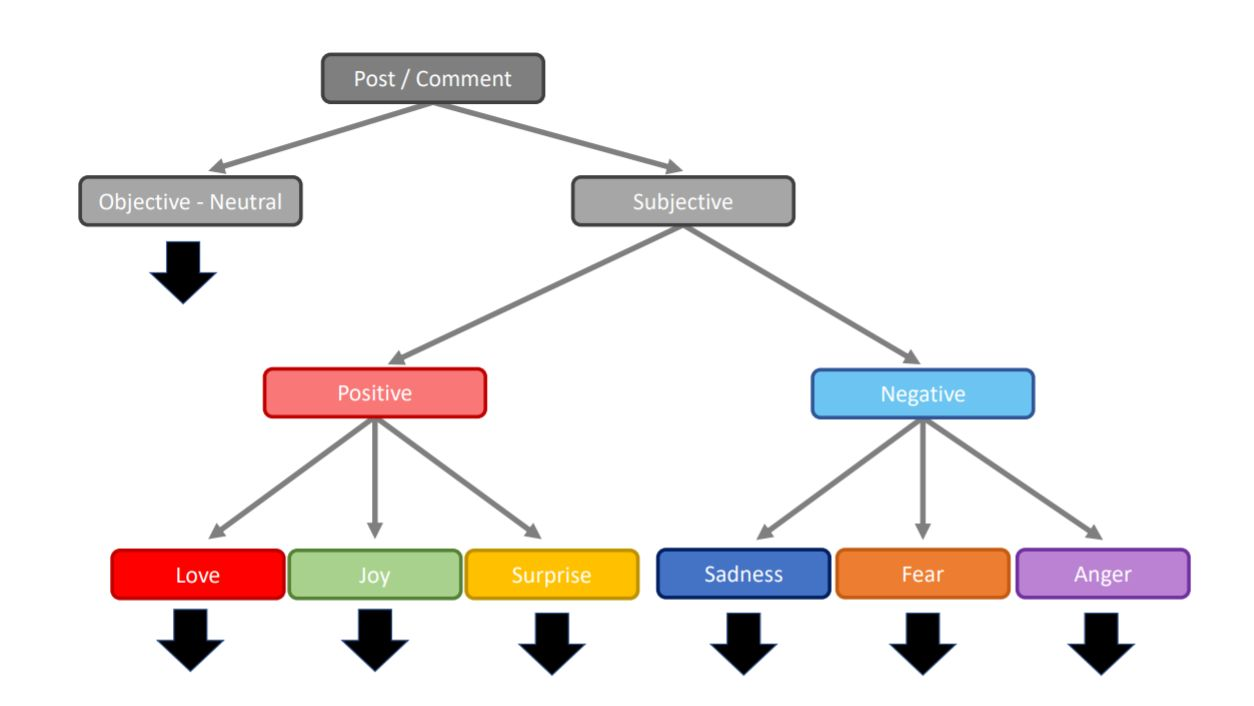
\includegraphics[width=0.4\linewidth]{imgs/classificatore-gerarchico}
    \caption{classificatore gerarchico}
    \label{fig:classificatore_gerarchico}
\end{figure}

\subsubsection{NLP Tasks: Part-Of-Speech tagging(PoS tagging)}
Processo nel quale le parti del testo vengono catalogate in nomi, pronomi, verbi ecc.

\subsubsection{NLP Tasks: Named Entity Recognition(NER)}
Riconoscere i nomi propri nel testo(persone, cose, luoghi ecc).

Può classificare anche seti di parole.

Si può usare NER in contesti specifici(droghe, condizioni mediche, reiferimenti bibliografici ecc).

\subsection{Sequence Data}

Una caratteristica ignorata fino ad ora è la sequnzialità dei dati,
come si comportano nel tempo?

Per alcuni campi questo aspetto serve:
\begin{itemize}
    \item \textbf{time series}: serie di valori ottenute a tempi successivi
    spesso con intervalli simili fra di loro
    \item \textbf{Natural lenguage processing}: le sequnze di parole in una frase hanno un significato
\end{itemize}


\subsection{Sliding window to analyze sequence data}
Per estrarre i dati da una sequenza, usiamo la sliding window.
Dove prendiamo una porzione dei dati, con la prissima sliding window prenderemo
porzione successiva(spesso si fa un overlapping del 50$\%$).

Si possono fare statistiche e applicare modifica del segnale nella sliding window che stiamo
analizzando:
\begin{itemize}
    \item media, deviazione standard, trasformata di fourir
\end{itemize}

Si può fare il sampling come se fosse un segnale analogico tradizionale
e ogni campione rappresenta una features del esempio.

\subsection{Testo come sequenza}
La sliding window può essere vista come le frasi che compongono il testo.

Non si fa campionamento perchè le parole sono una misurazione discreta.

\subsection{Modello Bag-Of-Word(BoW)}
\begin{itemize}
    \item creiamo un vocabolario con tutte le parole ed encodiamo le frasi con vettori
    binari
    \item la dimensione del vettore è la stessa del vocabolario, ogni componenete del vettore
    è una features.
    \item si possono ragruppare parole per avere features più sofisticate
\end{itemize}

\begin{figure}[H]
    \centering
    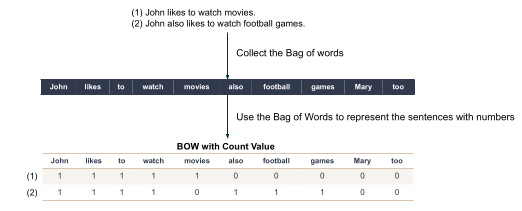
\includegraphics[width=0.7\linewidth]{imgs/bow}
    \caption{BoW}
    \label{fig:BoW}
\end{figure}


\subsection{Normalizzazion del testo}
\begin{enumerate}
    \item Vogliamo separare le paarole(task di tokenizzazione)
    \item Magari vogliamo considerare alcuni casi come gruppi di parole e non
    come parole singole
\end{enumerate}

\subsubsection{Primo problema di BoW}
\begin{itemize}
    \item l'encoding del vettore per ogni parola dipende dal vocabolario
    \begin{itemize}
        \item problemi con le lingue e si rischia la course of dimensionality
    \end{itemize}
    \item mentre si processa il testo, dobbiamo preoccuparci di ridurre il numemro di parole
    che prendiamo in considerazione
\end{itemize}

Possiamo seleionare un numero massimo di features e solo le parole più frequenti vengono
encodate.

\subsubsection{Stopwords}
\begin{itemize}
    \item se consideriamo le parole più frequenti probabilmente terremo le parole
    più usate di una lingua(non utile)
    \item solitamente si rimuovono le \textbf{stopwords(parole più comuni di una lignua)}
\end{itemize}

\subsubsection{Lemmatization and Stemming}
Il \textbf{lemmatization} è il procedimento dove parole con la stessa radice vengono riconosciute
anche se hanno una superficie diversa.

Spesso questa task si fa con una mappa associativa fornita dall'utente.

lo \textbf{Stemming} si riferisce ad una versione semplificata della lemmatization
dove semplicemente si elimano i suffissi dalle parole.

\subsubsection{Gli N-grammi possono essere dispendiosi}
Usare n-grammi maggiori di 3 è troppo dispendioso computazionalmete.

Spesso alcune parole vengono encodate insieme per rispramiare risorse.

Un idea è distinguere il ruolo di una parola nella frase.


\subsubsection{limiti di BoW}
BoW rappresenta le parole come simboli discreti e definisce rappresentazioni locali.

Le aprole sono rappresentate indipendentemente dal contesto, ordine e frequenza con
l'encoding, il che rende difficile trovare similarità.

\subsubsection{TF-IDF}
TFIDF(Term Frequency–Inverse Document Frequency), è una statistica
numerica che vuole riflettere quanto una parola è importante in un documento.


\begin{figure}[H]
    \centering
    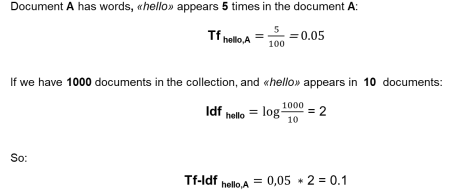
\includegraphics[width=0.7\linewidth]{imgs/tf-idf}
    \caption{TF-IDF}
    \label{fig:TF-IDF}
\end{figure}


\subsection{Toward Distributional Semantics}
\begin{itemize}
    \item BoW è una rappresentazione locale e non tiene conto di varie cose dipendentemente dalla task:
    \begin{itemize}
        \item ordine delle parole
        \item sinonimi
        \item contesto
        \item ortogonalità
        \item vettori con una dimensione poco informativi
    \end{itemize}
    \item usando TF-IDF basato su BoW si risolve parte del problema
    \begin{itemize}
        \item La dimensione dei vettori rimane un problema
        \item nessun ordine delle parole
        \item teniamo in conto che il contesto generale è più informativo delle 
        singole parole prese da sole
    \end{itemize}
\end{itemize}

\subsubsection{Distributional Semantics}
Il significato della parola dipende dalle parole che le stanno spesso vicine.

Quando una parola p appare nel testo, si analizzano le parole vicine.

usiamo tutte le parole vicine per imparare una rappresentazione della parola.

\begin{itemize}
    \item Cosa vogliamo fare:
    \begin{itemize}
        \item vettori dednsi per ogni parola, scelte in modo che parole di contesti simili
        abbiano vettori simili
        \item dimensionalità arbitraria del vettore di parole(dimensione come parametro)
        \item questo vettore basato sui differenti contesti delle parole del dataset lo
        vogliamo imparare con un approccio data driven
    \end{itemize}
    \item I vettori di parole vengon chiamati \textbf{word embeddings}
\end{itemize}

\subsection{Word2Vec}
\begin{itemize}
    \item Algoritmo per imparare vettori di parole che sfrutta le reti neurali artificiali
    (chiamato embedding)
    \item Per imparare i vettori che rappresentano le praole, volgiamo tener conto del contesto
    delle parole circostanti
    \item L'obbiettivo è allenare una ANN a prevedere un contesto da una parola data
    \item dovremmo allenare una rete particolare(ma semplice) che ha gli stessi layer di
    input e output con un layer di compressione in mezzo.
\end{itemize}

\begin{figure}[H]
    \centering
    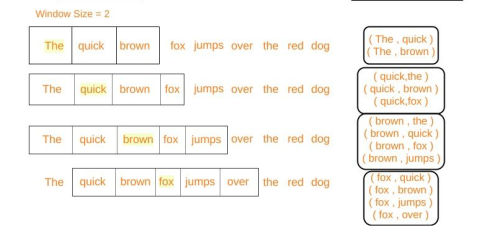
\includegraphics[width=0.7\linewidth]{imgs/esempio-word2vec}
    \caption{esempio Word2Vec}
    \label{fig:esempio_Word2Vec}
\end{figure}


\subsubsection{Encoder-Decoder architecture}
avendo le due frasi:
\begin{itemize}
    \item The King is sleeping in the castle
    \item The Queen is walking in the castle
\end{itemize}

E supponendo di prendere 5 parole per il contesto(grandezza della window).

Quindi se gli do in pasto king, dovrebbe saper predirmi {The, is, sleeping, in, castle}.


\begin{figure}[H]
    \centering
    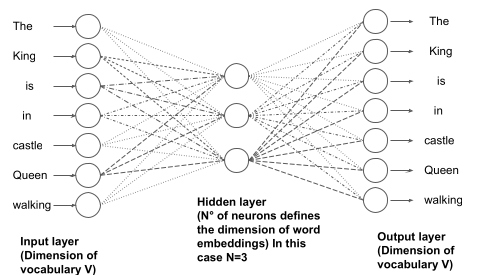
\includegraphics[width=0.7\linewidth]{imgs/encode-decode1}
    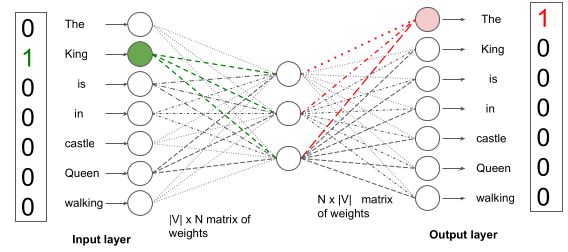
\includegraphics[width=0.7\linewidth]{imgs/encode-decode2}
    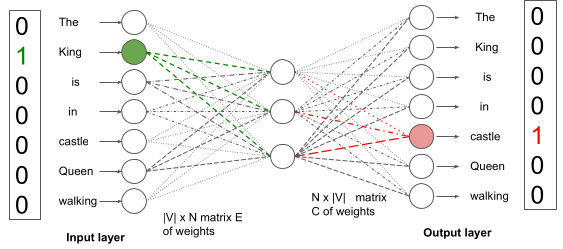
\includegraphics[width=0.7\linewidth]{imgs/encode-decode3}

    \caption{Encode decode}
    \label{fig:encode-decode1}
\end{figure}


\subsubsection{Skip-gram model in generale}


\begin{figure}[H]
    \centering
    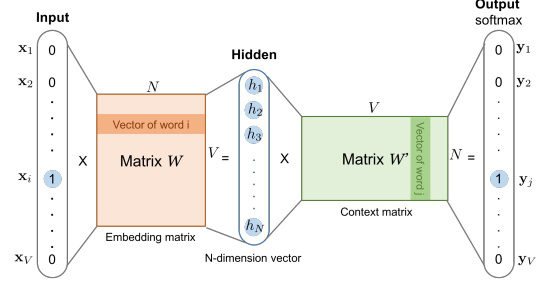
\includegraphics[width=0.7\linewidth]{imgs/skip-gram-model}
    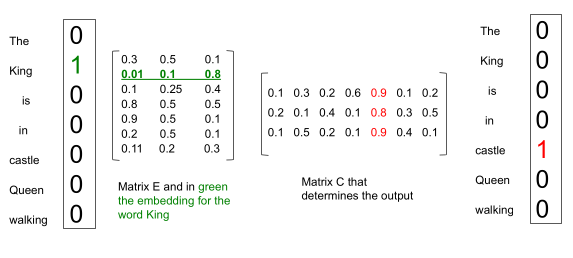
\includegraphics[width=0.7\linewidth]{imgs/skip-gram2}
    \caption{Skip-gram}
    \label{fig:Skip-gram}
\end{figure}



\subsubsection{Word2Vec formalmente}
\begin{itemize}
    \item Ogni parola dentro ad un vocabolario prefissato deve essere rappresentata
    da un vettore con dimensioni arbitrarie
    \item per ogni posizione \textbf{t} nel testo si considera di imparare aa predirre
    le parole attorno alla parola nel contesto
    \item formalmente stiamo calcolando la probabilità che una parola che una parola
    sia presente vicino alla parola data da cercare
    \item continuo a migliorare il vettore della parola per migliorare la resa(probabilità di pigliarci)
\end{itemize}





































